\chapter{Экспериментальное исследование параметров устройства квантовой коммуникации с недоверенным приемным узлом} \label{ch:ch5}
\section{Интерференция сигналов на боковых частотах фазомодулированного излучения} \label{sec:ch5/sec1}

Для проверки концепции была собрана оптическая схема, представленная на рисунке \ref{fig:RF_sin}. Для простоты использовался только один источник излучения, сигнал на выходе которого делился светоделителем 50:50 $СД1$. Такой подход позволяет имитировать случай, когда у Алисы и Боба хорошо скоррелированные источники излучения. В данном эксперименте применялся лазер с распределенной обратной связью Л1 (TTX1994 Neophotonics), отличительными особенностями которого являются очень узкая ширина спектральной линии порядка 100~кГц и широкий диапазон перестройки длин волн (от 1530~нм до 1565,5~нм) с высокой степенью точности (20~пм). Выходная мощность при этом составляла 10~мВт. Однако, это значение зависит от глубины динамического диапазона перестраиваемого оптического аттенюатора ПОА и суммарных потерь, вносимых элементами Алисы или Боба, так как результирующая мощность сигнала на боковых частотах должна не превышать величину 2,56~пВт, соответствующую среднему числу фотонов в импульсе 0,2 при частоте смены состояний 100~Мгц.   

Из-за чувствительности резнатора внутри лазера с распределенной обратной связью к обратному относительно выходного оптическому излучению, то есть переотражениям и рассеиванию сигналов, в оптической схеме применяется волоконный изолятор И на основе эффекта Фарадея с величиной изоляции порядка 50~дБ. Для перевода системы в однофотонный режим применяется ПОА с достаточной малым шагом перестройки 0,05 дБ и большим динамическим диапазоном величиной 60~дБ.  

 \begin{figure}[ht]
  \centering
  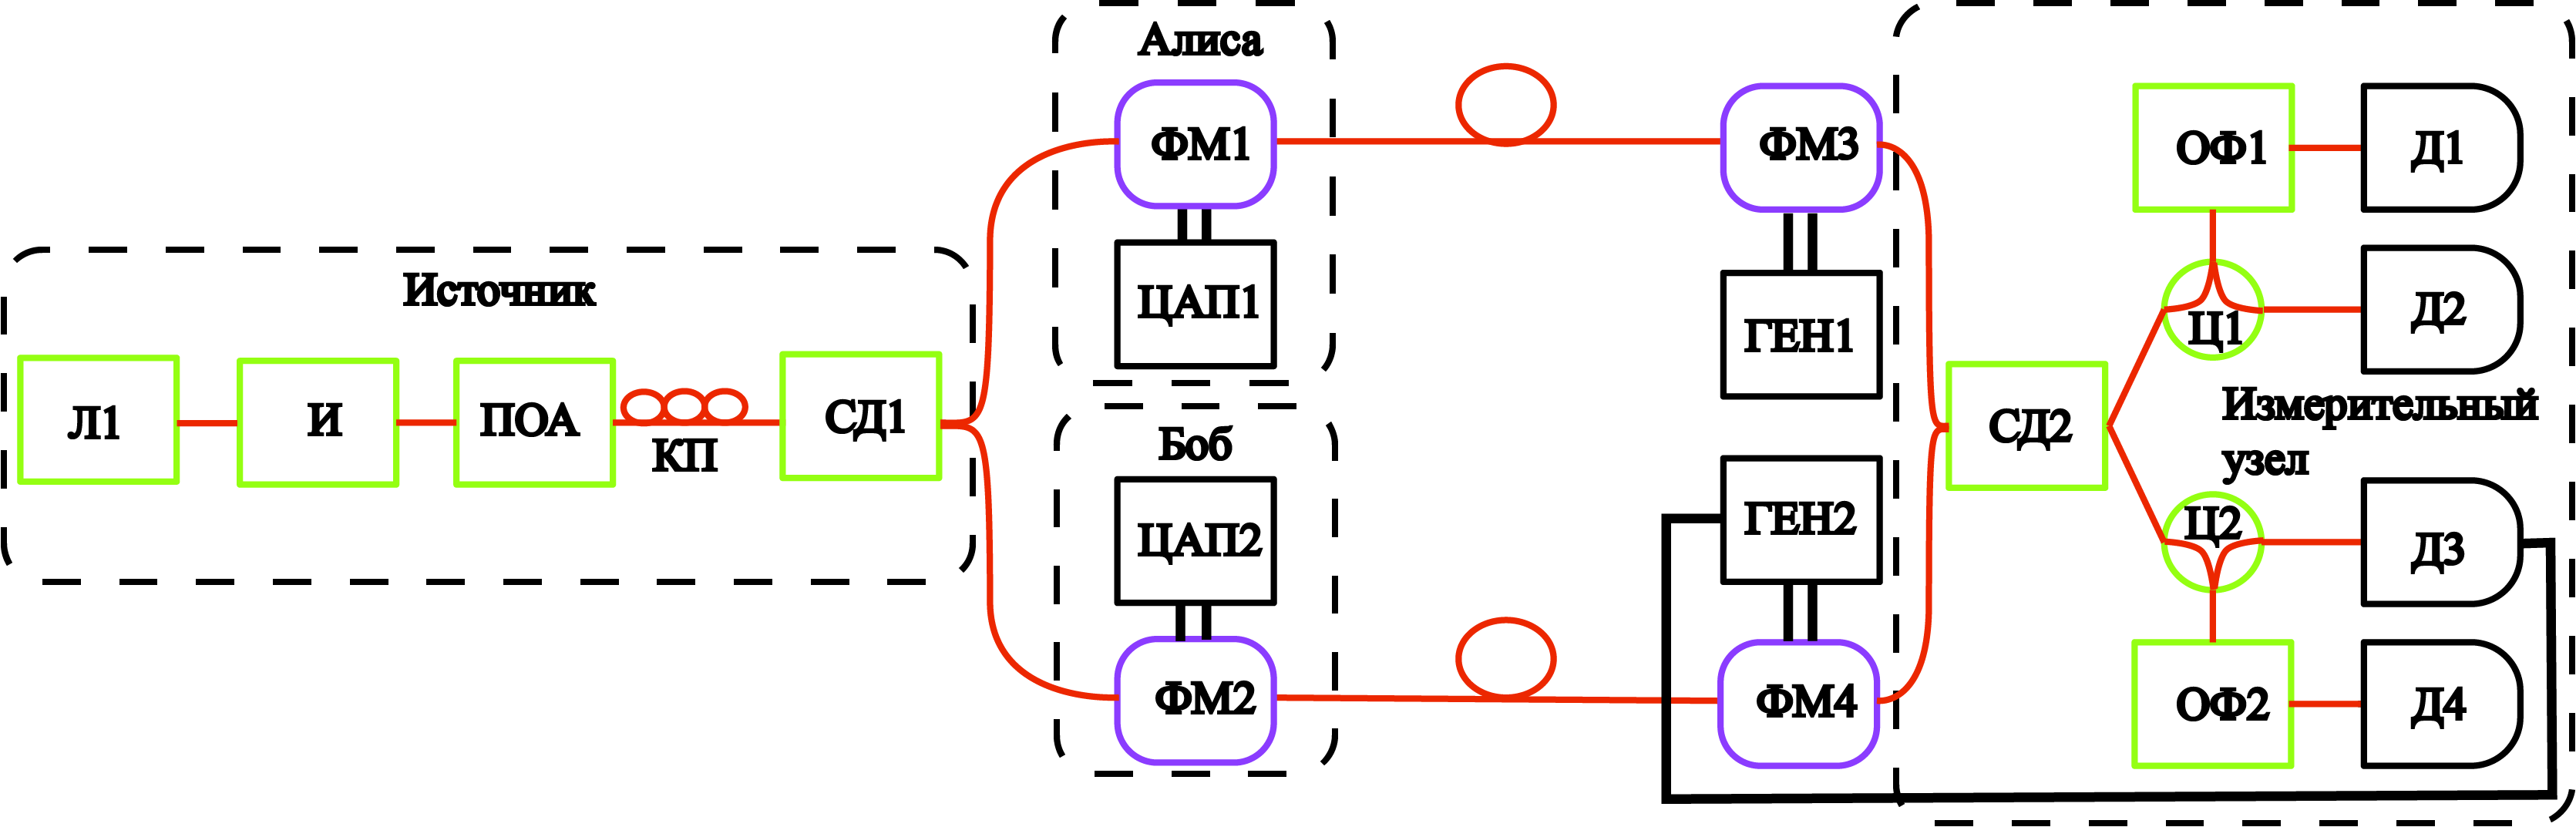
\includegraphics[scale=0.5]{Scheme_colored_rus.png}
  \caption{Принципиальная схема экспериментального стенда}
  \label{fig:RF_sin}
\end{figure}

На выходе из источника сигнал проходил по двум плечам формируемого таким образом интерферометра через светоделитель, благодаря чему имитировалось, что Алиса и Боб - это раздельные узлы, в которых информация кодировалась с помощью фазовых модуляторов. Выходы первого светоделителя подключались ко входам двух независимых 10~ГГц электро-оптических модуляторов на основе $LiNbO_3$ (со встроенным поляризатором) $ФМ1$ and $ФМ2$. Поляризаторы снижали чувствительность модуляторов к поляризации входного излучения, для чего использовался контроллер поляризации КП, и таким образом, повышалась видность картины интерференции. Электрические входы $ФМ1$ и $ФМ1$ подключались к выходам с цифро-аналоговых преобразователей ЦАП с модулирующим радиочастотным синусоидальным сигналом (с частотой 4,8~ГГц). Амплитуды управляющих сигналов подбирались таким образом, чтобы мощность сигнала на боковых частотах была равно у Алисы и у Боба. 

% and provide 0.2 photons intensity of sidebands.

Индекс модуляции, который показывает долю энергии на боковых частотах по отношению к центральной в результате модуляции должен быть 5~\%. В таком случае наблюдается оптимальное соотношение сигнала на боковых частотах к шуму проходящей через оптический фильтр центральной частоты.  Так что средняя величина оптической мощности была равна 2.56~пВт, что соответствует $\mu=0.2$.  


В данном исследовании  использовались только два кодирующих фазовых состояния на Алисе и Бобе ($\varphi_{A,B}\in\{0,\pi\}$. Разница фаз ($\Delta\varphi$) между Алисой и Бобом формировалась с помощью изменения IQ-таблиц ЦАП при помощь ПЛИС и ПО сосбтвенной разработки. В случае измерения зависимости количества срабатываний детекторов от разности фаз ($\Delta\varphi$) фаза сдвигалась последовательно с шагом $\varphi_{step}\ = 10^{\circ}$. Наблюдаемые состояния на выходах $ФМ1$ и $ФМ2$ могут быть описаны в соотвествии с уравнением~\ref{phi}.

После того, как состояния приготовлены, мы посылаем их в квантовый канал. Для компенсации оптической разности хода в двух плечах интерферометра, а так же для точной подстройки оптических фаз сигналов использовались $ФМ3$ и $ФМ4$. Эта подстройка осуществлялась при помощи изменения постоянного напряжения, подаваемого на модуляторы и формируемого двумя независимыми электрическими выходами генератора сигналов $GEN1$ и $GEN2$. Выходы втрой пары фазовых модуляторов подключались к паре входных портов светоделителя $СД2$ 2x2 с коэффициентом деления 50:50.

Измерения проводились в два этапа: первый этап в классическом свете, второй этап - в режиме счета фотонов на сверхпроводниковом детекторе одиночных фотонов (Сконтел), у которого встроены два независимых приёмника $Д1$, $Д4$. Квантовая эффективность обоих была равна 10~\%, а уровень темновых шумов не превышал 50~Гц для каждого. Измеренная величина суммарных шумов, включающих в себя темновые срабатывания и засветку от центральной частоты в силу ограниченной экстинкции оптического фильтра, составляла $\gamma_{темн}=1.5$ кГц.

Фотография экспериментального стенда представлена на рисунке \ref{fig:experimental_setup_TF}.  

 \begin{figure}[ht]
  \centering
	 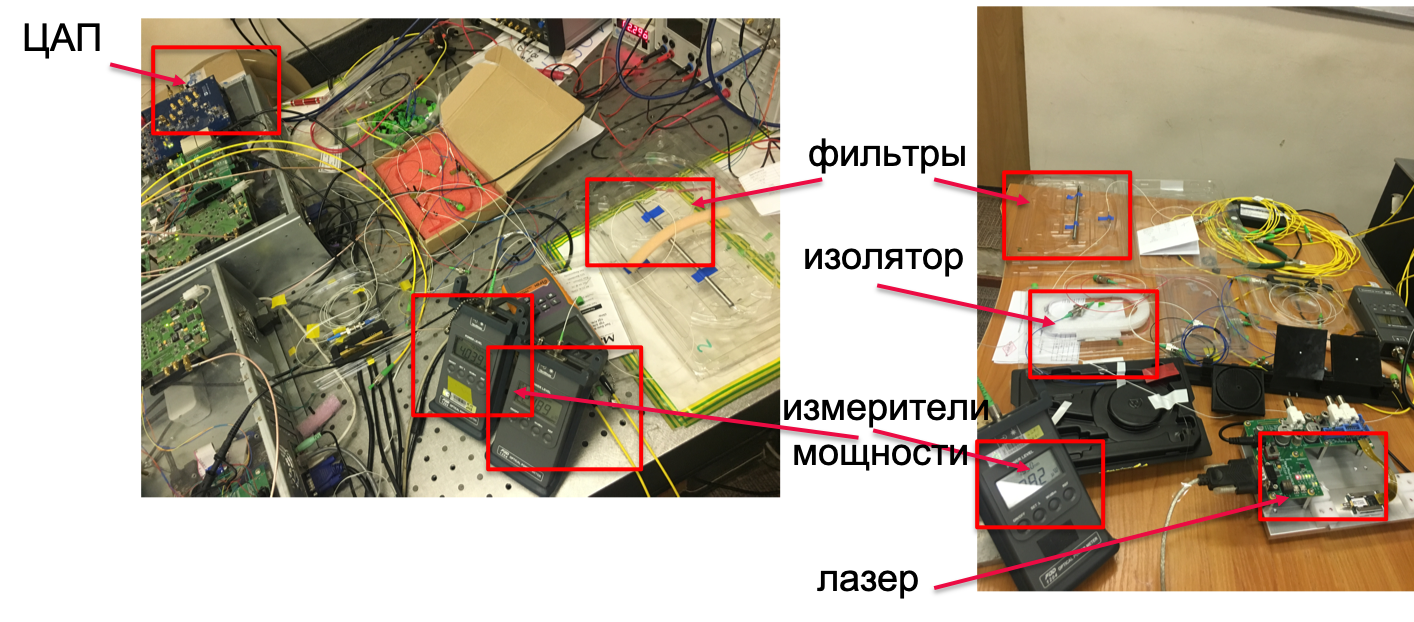
\includegraphics[scale=0.7]{Experimental_setup_TF}
  \caption{Фотография экспериментального стенда}
  \label{fig:experimental_setup_TF}
\end{figure}

\pagebreak

%%%%%%%%%%%%%%%%%%%%%%%%%%%%%%%%%%%%%%%%%%%%%%%%%%%%%%%%%%%%%%%%%%%%%%%%%%%%%%%%%
\section{Характеристики компонентов экспериментального стенда} \label{ch:ch5/sec2}

Значительную трудность представляет согласование спектральных характеристик Алисы и Боба. Даже при использовании одного источника для имитации хорошо скоррелированных лазеров, требуется подобрать оптические фильтры с максимально совпадающими характеристиками. В системе квантовой коммуникации частота модулирующего сигнала равна $\Omega = 4,8$~ГГц (рис.\ref{fig:RF_sin_osc} ). Значит, полоса спектрального фильтра не должна превышать величину $2\Omega$. Для этих целей используются волоконные узкополосные оптические фильтры на основе Брэгговских решеток. На рисунке \ref{fig:Spectrums} показаны измеренные характеристики максимально близких по серединному значению полосы пропускания фильтров. Уровень полуширины (FWHM) первого фильтра ОФ1 равен 48,8~пм (или 6,1~ГГц), а уровень полуширины (FWHM) второго фильтра ОФ2 равен 40~пм (или 5~ГГц). При этом разность центральных длин волн составляет 8~пм (или 1~ГГц). В ходе эксперимента лазер подстраивался таким образом, чтобы минимальная величина засветки от центральной проходила через оба оптических фильтра. Из-за несовпадения их характеристик повышался уровень шумов, вследствие чего ухудшалась видность картины интерференции.  

 \begin{figure}[ht]
  \centering
  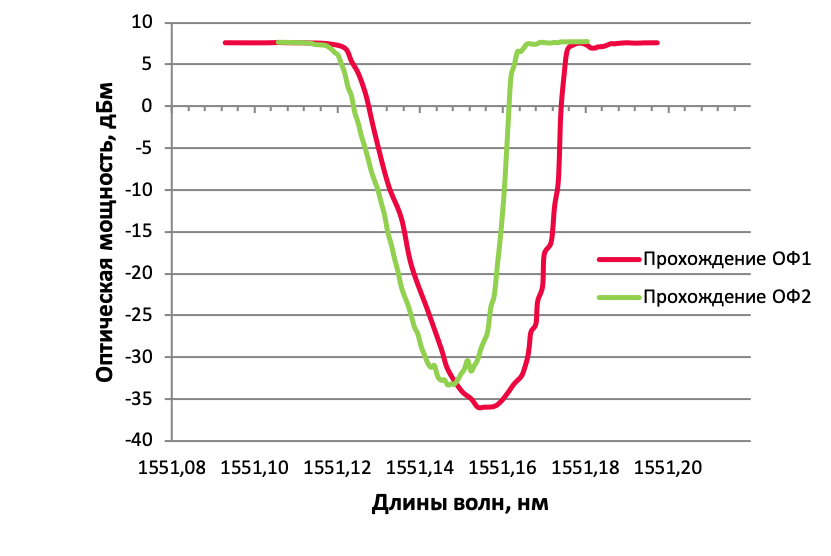
\includegraphics[scale=0.8]{T-spectrums.png}
  \caption{Спектральные характеристики оптических фильтров}
  \label{fig:Spectrums}
\end{figure}

\pagebreak

%%%%%%%%%%%%%%%%%%%%%%%%%%%%%%%%%%%%%%%%%%%%%%%%%%%%%%%%%%%%%%%%%%%%%%%%%%%%%%%%%%%%%%%%%%%%%%%%%%%%%%%%%%%%%%%%%
%\section{Экспериментальный стенд} \label{ch:ch5/sec3}


%\pagebreak

%%%%%%%%%%%%%%%%%%%%%%%%%%%%%%%%%%%%%%%%%%%%%%%%%%%%%%%%%%%%%%%%%%%%%%%%%%%%%%%%%%%%%%%%%%%%%%%%%%%%%%%%%%%%%%%%%
\section{Зависимость интенсивности на боковых частотах от сдвига фаз в результате интерференции в классическом режиме} \label{ch:ch5/sec5}


На первом этапе измерения проводились в классическом режиме с помощью измерителей оптической мощности и нулевом значении вносимых потерь ПОА. При этом один из измерителей мощности $Д3$ служил для обратной связи и подстройки оптической фазы между двумя плечами с помощью $ФМ4$ и $ГЕН2$. Когда разность оптических фаз была скомпенсирована, и центральная мода постоянно наблюдалась в одном из выходных плечей $СД2$, в ручном режиме последовательно производилась смеша фазовых состояний радиочастотных модулирующих сигналов посредством изменения значений в IQ-таблице ЦАПов с шагом $10^{\circ}$. 

В результате наблюдалась картина на рисунке \ref{fig:Experimental_TF_classical}. Значение конструктивной интерференции на первом детекторе составило величину $I_{max}=6,3$~мкВт, а деструктивной -- $I_{min}=0,2$~мкВт, тогда как на втором $I_{max}=6,13$~мкВт, и $I_{min}=0,08$~мкВт, соответственно. 

 \begin{figure}[ht]
  \centering
  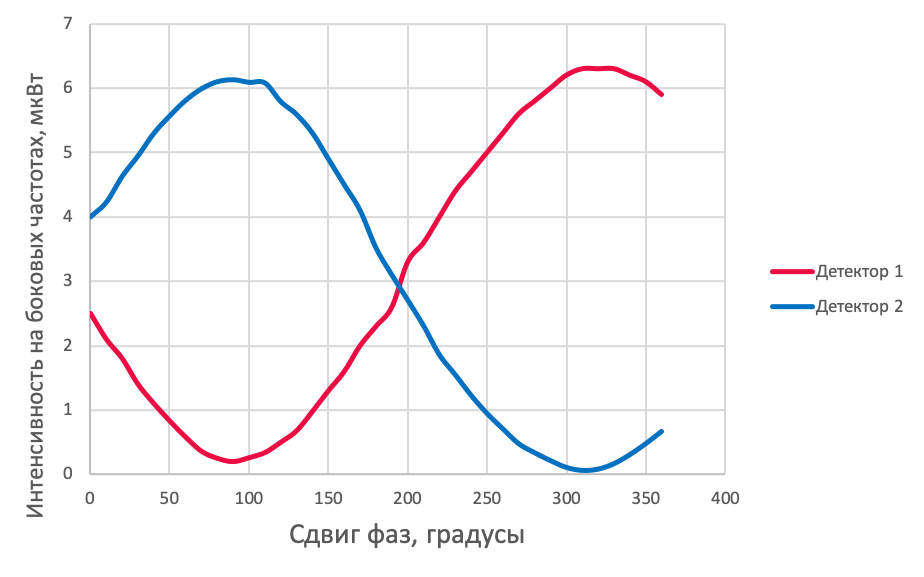
\includegraphics[scale=0.7]{Experimental_TF_classical.png}
  \caption{Зависимость интенсивности на боковых частотах в результате интерференции от разности фаз модулирующих сигналов}
  \label{fig:Experimental_TF_classical}
\end{figure}

Если определить отношение $I_{max}$ к $I_{min}$, как контраст, то в первом плече контраст был равен 31,5, а во втором -- 76.6. Видность интерференционной картины определяется как: 
\begin{equation}
	V=\frac{I_{max}-I_{min}}{I_{max}+I_{min}}
\end{equation}

В первом случае видность составила $V_{1}=93,8\%$, во втором -- $V_{2}=97,4\%$


\pagebreak

%%%%%%%%%%%%%%%%%%%%%%%%%%%%%%%%%%%%%%%%%%%%%%%%%%%%%%%%%%%%%%%%%%%%%%%%%%%%%%%%%%

\section{Вероятности срабатываний детекторов} \label{ch:ch5/sec6}

 Известно, что оптический фильтр отражает центральную оптическую моду ($k=0$). Значит, среднее число фотоном на входе в каждый детектор может быть найдена как \ref{nph1}. 
 
\begin{align}\label{nph1}
    n(\Delta\varphi)_{1,2}&=\mu_0\eta_c\Bigg(\sum_{k\neq 0}|d_{0k}^{S}(\beta)|^2 + \vartheta|d_{0k}^{S}(\beta)|^2 \pm \nonumber \\
    &\pm \cos(\varphi_0)\Big(\sum_{k\neq 0}|d_{0k}^{S}(\beta)|^2e^{i\Delta\varphi k}+ \vartheta|d_{0k}^{S}(\beta)|^2 \Big) \Bigg),
\end{align}

где $\Delta\varphi=\varphi_B-\varphi_A$, $\varphi_0$ это относительная оптическая фаза между импульсами отправителя (Алисы) и получателя (Боб), $\vartheta \ll 1$ часть центральной моды ($k=0$) проходящая через фильтр, ввиду ограниченности его характеристики. Используя свойства d-функци из \cite{varshalovich1988quantum}, можно упростить предыдущее выражение \ref{nph}

\begin{align}
    n(\Delta\varphi)_{1,2}=\mu_0\eta_c\Big(1-(1-\vartheta)(1\mp\cos(\varphi_0))|d_{00}^{S}(\beta)|^2 \pm \nonumber \\
    \pm\cos(\varphi_0)d_{00}^{S}(\beta')\Big) \label{nph},
\end{align}

где аргумент $\beta'$ получен следующим образом \ref{betaappox}. 

\begin{equation} \label{betaappox}
    \cos(\beta')=\cos^2(\beta) \mp \sin^2(\beta)\cos(\Delta\varphi).
\end{equation}

Чтобы оценить вероятность срабатывания воспользуемся линейным приближением Манделя, предполагая слабые интенсивности ($n(\Delta\varphi)_{1,2} \ll 1$):

\begin{eqnarray}
    \mathcal{P}_{1,2}^{+}(\Delta\varphi)=\left(n(\Delta\varphi)_{1,2}\eta_DF+\gamma_{dark}\right)\Delta t, \label{pdet}
\end{eqnarray}

где $\eta_D$ квантовая эффективность, $F$ частота смены состояний, $\gamma_{dark}$ частота темновых отсчетов детектора одиночных фотонов, и $\Delta t$ время окна срабатывания. Для простоты положим $\Delta t F=1$. Отсутствие срабатывания определим, как $\mathcal{P}_{1,2}^{-}(\Delta\varphi)=1-\mathcal{P}_{1,2}^{+}(\Delta\varphi)$.     


Используем несколько полезных приближений, которые помогут оценить квантовый коэффициент ошибок по битам (QBER) и скорости формирования просеянного ключа. Для начала положим, что число взаимодействующих мод велико ($S\rightarrow \infty$), что действительно так для стандартных волоконно-оптических модуляторов. Тогда можно использовать приближение d-функций следующим образом:

\begin{align}
d_{nk}^S(\beta) &\xrightarrow{S\rightarrow \infty} J_{n-k}(m), \label{limdj} \\
\beta &\propto m, \label{propto}
\end{align}
где $J_k(m)$ функция Бесселя первого порядка. Полагая значение $m$ малым, что действительно так, в соотвествии с теорией классической модуляции воспользуемся приближением первого порядка функции Бесселя. 


Так в соответствии с уравнение \ref{betam} $\beta \rightarrow 0$, следовательно можно использовать аппроксимации первого порядка для выражения \ref{betaappox} в терминах $m$ подразумевая пропорциональность в уравнении \ref{propto}.


Определим уравнение~\ref{pdet} следующим образом:

\begin{align}\label{pdet1}
 \mathcal{P}_{1,2}^{+}(\Delta\varphi)&=\mu\eta\Big(1\pm\cos(\Delta\varphi)\cos(\varphi_0)\Big)+ \nonumber
 \\
 &+\vartheta\Big(\mu_c\eta(1\pm\cos(\varphi_0))\Big)+p_{dark},
\end{align}


где $\eta$ полная оптическая пропускная способность квантового канала с учетом квантовой эффективности детектора, $p_{dark}=\gamma_{dark}\Delta t$ это вероятность темнового срабатывания во временном интервале $\Delta t$, и $\mu$ и $\mu_c$ это среднее число фотонов на боковых и на центральной моде соотвественно после модуляции, как определено:

\begin{align}
    \mu&=\mu_0\sum_{k\neq 0}|d_{0k}^{S}(\beta)|^2, \\
    \mu_c&=\mu_0-\mu=\mu_0(1-\sum_{k\neq 0}|d_{0k}^{S}(\beta)|^2).
\end{align}
Выраение в уравнени~\ref{pdet1} даёт точное соотношение между экспериментальными параметрами и показывает, как они влияют на вероятности детектирования квантовых состояний. 


\pagebreak

%%%%%%%%%%%%%%%%%%%%%%%%%%%%%%%%%%%%%%%%%%%%%%%%%%%%%%%%%%%%%%%%%%%%%%%%%%%%%%%%%%
\section{Зависимость интенсивности на боковых частотах от сдвига фаз в результате интерференции в режиме счета фотонов} \label{ch:ch5/sec7}



 \begin{figure}[ht]
  \centering
  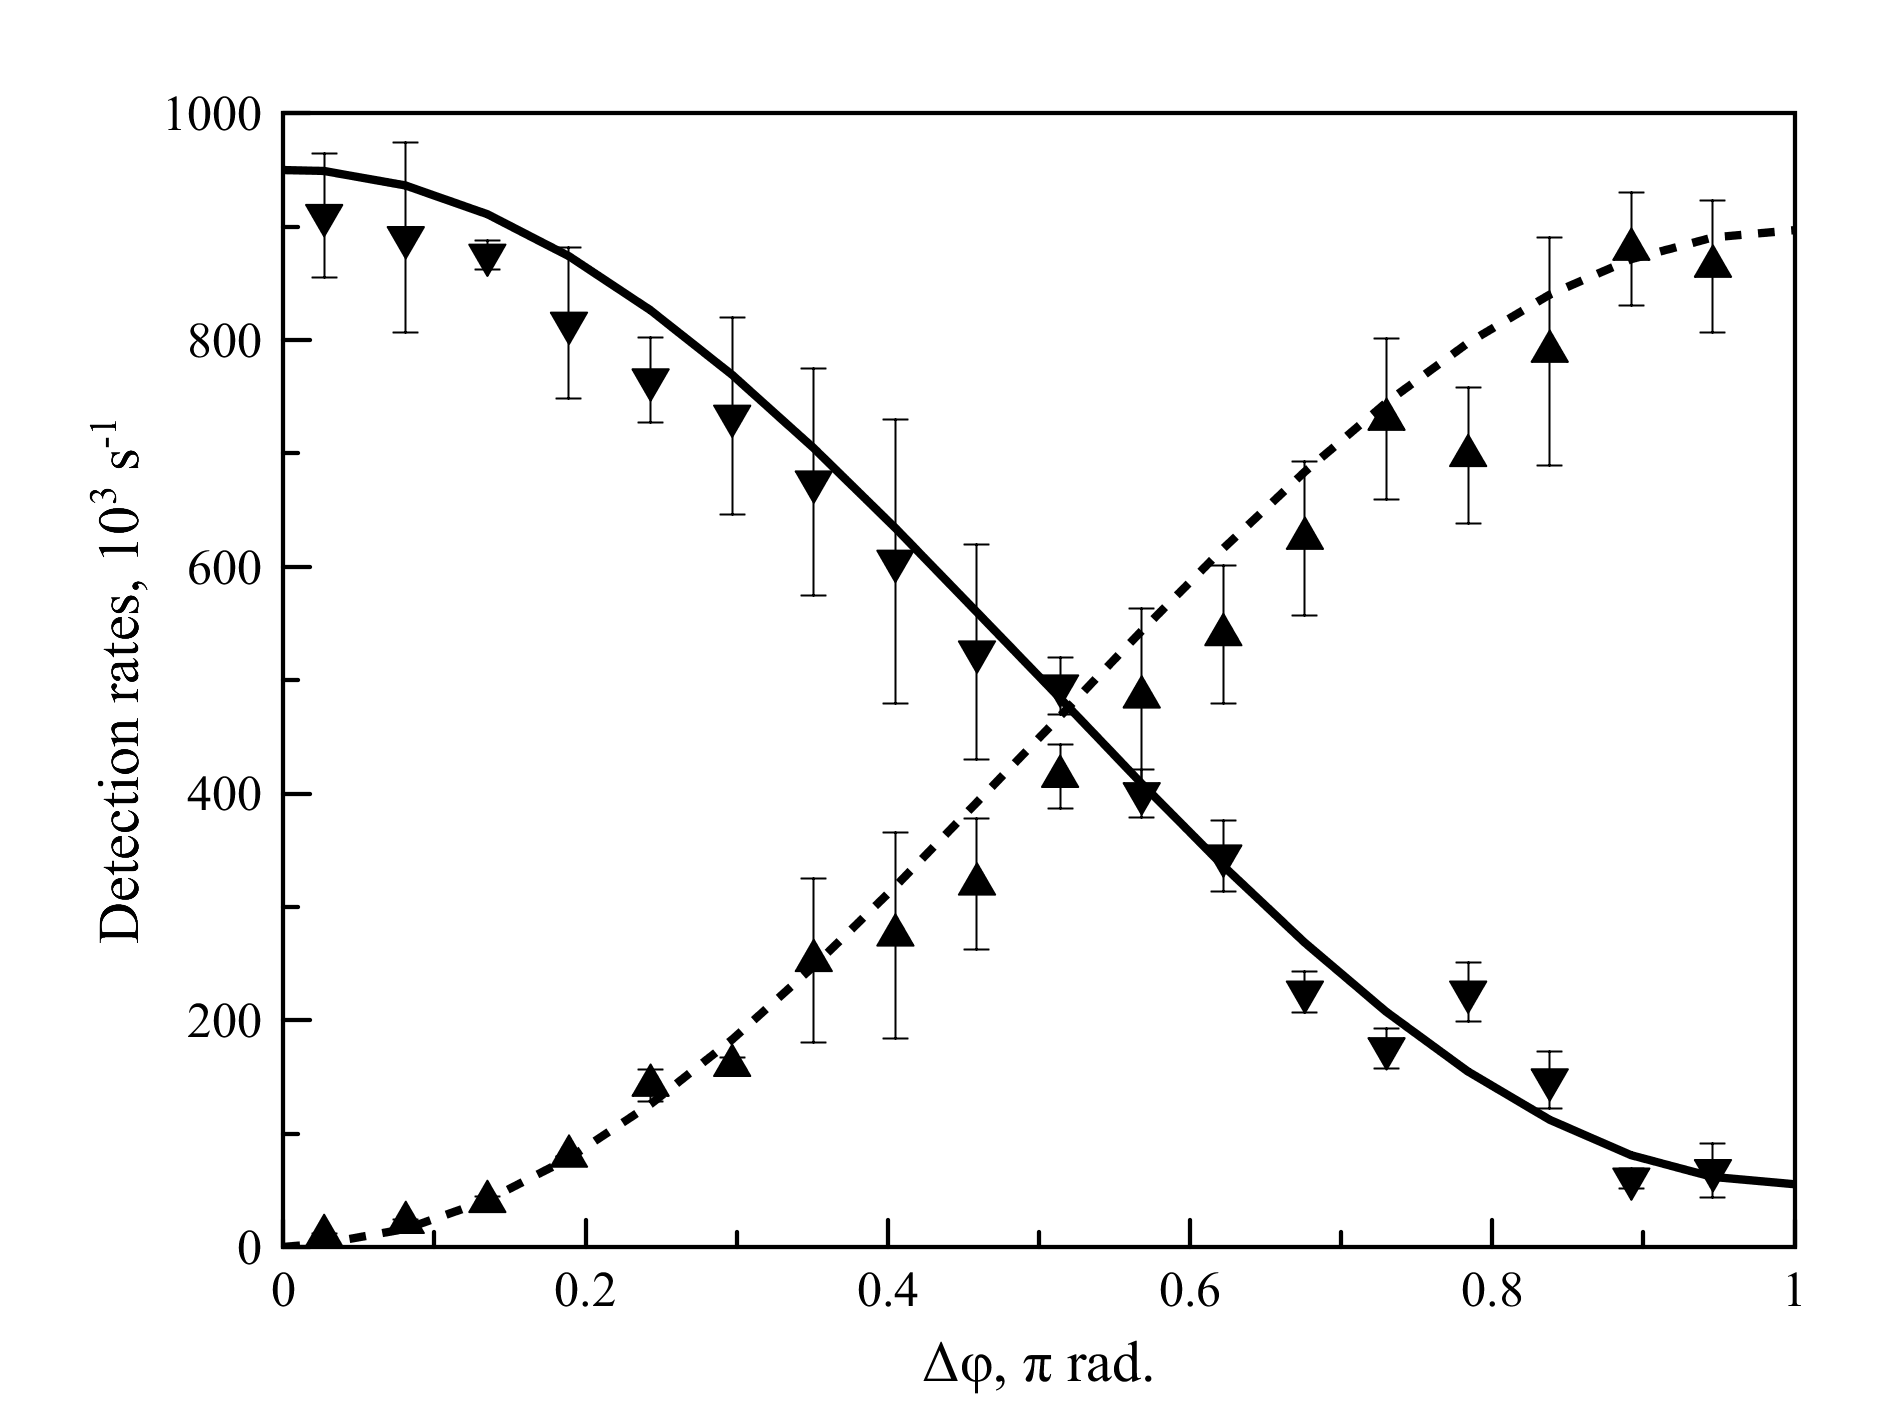
\includegraphics[scale=0.2]{ExperimentTF.png}
  \caption{Зависимость количества отсчетов в результате интерференции от разности фаз модулирующих сигналов}
  \label{fig:Experimental_TF}
\end{figure}


\pagebreak

%%%%%%%%%%%%%%%%%%%%%%%%%%%%%%%%%%%%%%%%%%%%%%%%%%%%%%%%%%%%%%%%%%%%%%%%%%%%%%%%%%
\section{Оценка коэффициента битовых ошибок и скорости формирования ключа} \label{ch:ch5/sect8}

Далее рассмотрим только те случаи, где срабатывание происходит только на одном из детекторов в единицу времени.  Таким образом, вероятности срабатываний $R$ определяются как:

\begin{align}
    R&=\Big(\mathcal{P}_{1}^{+}\mathcal{P}_{2}^{-}(\Delta\varphi=\varphi_m)+\mathcal{P}_{1}^{-}\mathcal{P}_{2}^{+}(\Delta\varphi=\pi+\varphi_m)+ \nonumber \\
    &+\mathcal{P}_{1}^{+}\mathcal{P}_{2}^{-}(\Delta\varphi=\pi+\varphi_m)+\mathcal{P}_{1}^{-}\mathcal{P}_{2}^{+}(\Delta\varphi=\varphi_m)\Big),
\end{align}


где $\varphi_m$ средняя величина несоответствия фаз $\varphi_A$ и $\varphi_B$. Первые два слагаемых - это вероятности успешного определения битов легитимными пользователями, тогда как оставшиеся два слагаемых - вероятности смены бита на противоположный (bitflip) (полагая $\varphi_0 \approx 0$). Таким образом, можно определить выражение для QBER $Q$ следующим образом:

\begin{align}
    Q=\frac{\mathcal{P}_{1}^{-}\mathcal{P}_{2}^{+}(\Delta\varphi=\varphi_m)+\mathcal{P}_{1}^{+}\mathcal{P}_{2}^{-}(\Delta\varphi=\pi+\varphi_m)}{R}.
\end{align}


Наконец, можно определить выражение для оценки среднего значения скорости формирования просеянного ключа $K$ (одинаковые биты между легитимными пользователями, но коррелирующие с возможным результатом у злоумышленника, что требует проведения процедуры усиления секретности)
\begin{equation}
    K=FR(1-h(Q)),
\end{equation}
где $h(Q)$ это функция двоичной энтропии. 

\pagebreak

%%%%%%%%%%%%%%%%%%%%%%%%%%%%%%%%%%%%%%%%%%%%%%%%%%%%%%%%%%%%%%%%%%%%%%%%%%%%%%%%%%
\section{Выводы по главе} \label{ch:ch5/sec9}


В \ref{ch:ch5} главе показано, что в результате интерференции квантового фазомодулированного сигнала на боковых частотах на симметричном светоделителе в схеме квантовой рассылки ключа с узлом регистрации, независящим от легитимного пользователя, происходит спектральное разделение квантового сигнала и сигнала на центральной длине волны с их независимой регистрацией в разных плечах светоделителя. 

\pagebreak

